\documentclass[]{article}
\usepackage{graphicx}
\usepackage{amsmath}
\usepackage{amsfonts}
%opening
\title{SAGA\\Automatic Temperature Schedule}
\author{Nil Mamano, Wayne Hayes}


\begin{document}

\maketitle


\section{Introduction}

\subsection{Simulated annealing}
Simulated annealing is a generic optimization algorithm. It can optimize (find good solutions -- not necessarily the best) any problem for which the necessary elements can be defined: what constitutes a \textit{solution}, the \textit{objective function} to optimize, and a \textit{neighbor relationship} that dictates which solutions are similar.

The \textit{space of solutions} is the graph with all the possible solutions as vertices and where there are edges between neighbor solutions. If the solutions are ``heightened'' according to their quality or \textit{score} (the value of the objective function), then the space of solution looks like a landscape. In this landscape, we are looking for the highest points (if maximizing) or the lowest points (if minimizing). From now on, we assume that our goal is to maximize the objective function.

Given some solution as starting point, we can explore the space of solutions by ``walking'' through the edges, with the goal of reaching a good solution. There is a whole family of algorithms based on different strategies of how to do this walk (i.e., how to choose the next neighbor at each step). For instance, in the hill climbing algorithm (called so because of the analogy with the landscape) we always move towards neighbors that are better than the current solution. Since neighbor solutions are similar, this can be seen as taking the starting solution and progressively refining it until it can't be improved anymore.

The distinctive characteristic of simulated annealing is that it adds randomness to the search, allowing to move towards worse solutions. This allows it to reach regions of the solution space that deterministic algorithms could not. At each step, a neighbor is chosen at random. If it is better than the current solution, it is adopted as new current solution. Otherwise, it may still be adopted with a certain probability, which depends on what is called the \textit{temperature schedule}.

\subsection{Temperature schedule}

The score increment between the current solution $x$ and a neighbor solution $x'$ is defined as $\triangle E = f(x')-f(x)$, where $f$ is the objective function\footnote{The letter $E$ in $\triangle E$ comes from \textit{energy}, because simulated annealing is inspired on annealing, a metallurgy technique used to minimize the thermodynamic free energy of a material.}.
A critical component of simulated annealing is the probability to accept a worse solution, i.e., the case $\triangle E < 0$. We formalize it as follows:
$$P(\triangle E, t)=\begin{cases}
 1& \text{ if } \triangle E\geq 0 \\ 
 e^{\triangle E/t}& \text{ if } \triangle E < 0 
\end{cases}$$
where $t\in \mathbb{R^+}$ is a control parameter called \textit{temperature}. When $\triangle E < 0$, the probability $P(\triangle E, t)$ increases monotonically with $t$. Hence, by changing the value of $t$, we can affect the behavior of simulated annealing: with higher temperatures, the search is more random, while with lower temperatures, the search is more deterministic. For any fixed score increment $a$, we have that $\lim_{t\rightarrow 0} {P(a, t)}=0$, i.e., when temperature approaches 0 simulated annealing acts as hill climbing. On the other hand, $\lim_{t\rightarrow +\infty} {P(a, t)}=1$. In that case, simulated annealing accepts worse solutions as much as better ones. 

In addition, the probability $P(\triangle E, t)$ increases monotonically as a function of $\triangle E$. This means that it is more likely to accept worse solutions whose score is closer to the score of the current alignment.

Usually, the temperature changes dynamically as the algorithm advances. It begins very high, so that the search starts with a randomized behavior, and progressively declines, becoming more selective, until towards the end the temperature is so low that no worse solutions are accepted and the algorithm stagnates at a local maximum of the solution space. In order to achieve this behavior, we define the temperature as a function of the step or \textit{iteration}. A simulated annealing iteration consists of choosing a random neighbor solution of the current alignment and either accepting it as new current solution or keeping the original one.

The \textit{temperature schedule} is a function $T(i)$ that determines the value of the temperature at iteration $i$. It can be defined in many ways, the only requirement is that $T(i)>0$ for all $i\in\mathbb{N}\cup\{0\}$ (the first iteration is the 0th). A typical definition for the temperature that we adopt for the remaining of the paper is
$$T(i)=k\cdot\frac{1}{e^{\lambda i}}$$
where $k,\lambda\in \mathbb{R}^+$, are user-defined constant parameters. Note that at the first iteration, $0$, we have $T(0)=k$. Hence, $k$ is called the starting temperature. $T(i)$ decreases at an exponential rate, approaching $0$ assimptotically: $\lim_{i\rightarrow +\infty} T(i)=0$. The parameter $\lambda$, known as the decay rate, controls how quickly the temperature decreases towards zero (see Figures~\ref{fig:temp} and~\ref{fig:lambda}).

\begin{figure}
\centering
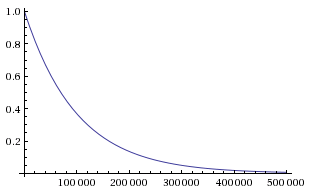
\includegraphics[width=0.99\linewidth]{../figures/plottemp}
\caption[Temperature schedule]{The temperature $T(i)$ as a function of the iteration $i$, with $k=1$ and $\lambda=0.00001$.}
\label{fig:temp}
\end{figure}

\begin{figure}
\centering
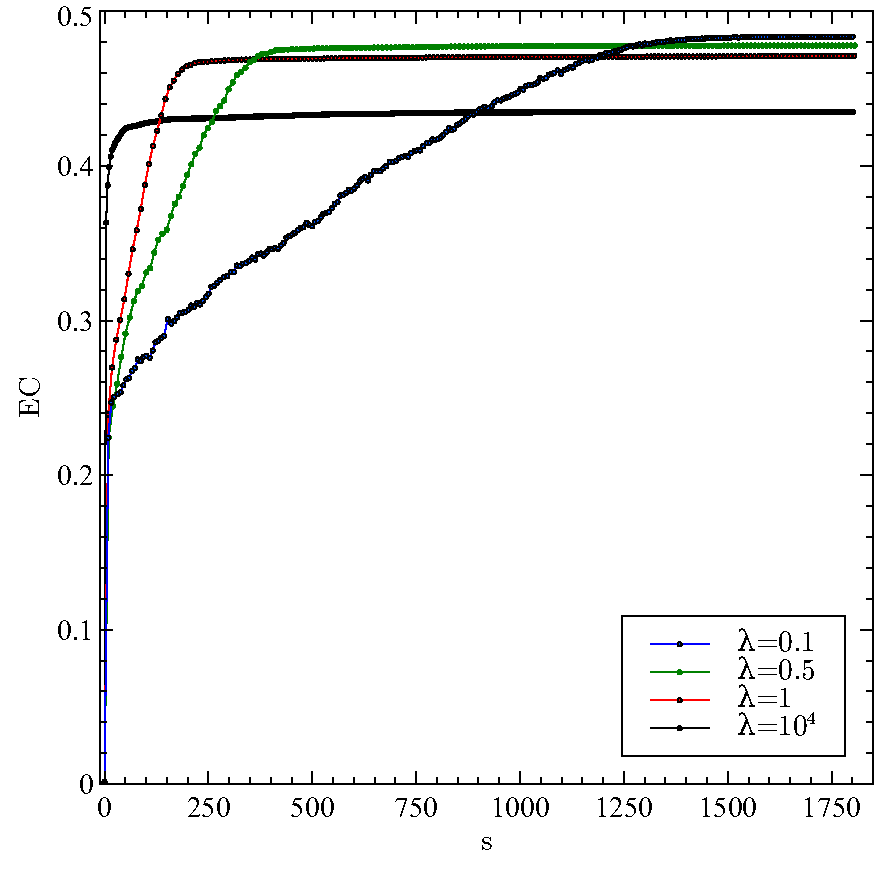
\includegraphics[width=0.8\linewidth]{../figures/lambda}
\caption[Temperature schedule: $\lambda$]{The effect of $\lambda$ in the convergence rate and quality of the final solution. Temporal progression of four 30-minute runs of SAGA with the networks from the Yeast and Human dataset, optimizing EC, with $k=4\cdot10^{-5}$ and different values of $\lambda$. The values of $\lambda$ shown are the original values multiplied by $10^{8}$.}
\label{fig:lambda}
\end{figure}

The parameters $k$ and $\lambda$ are necessary to adjust the temperature schedule (see Figure~\ref{fig:parameters}), which can affect the effectiveness of simulated annealing greatly. The goal of this paper is to set $k$ and $\lambda$ automatically depending on the characteristics of the solution space.

\begin{figure}
\centering
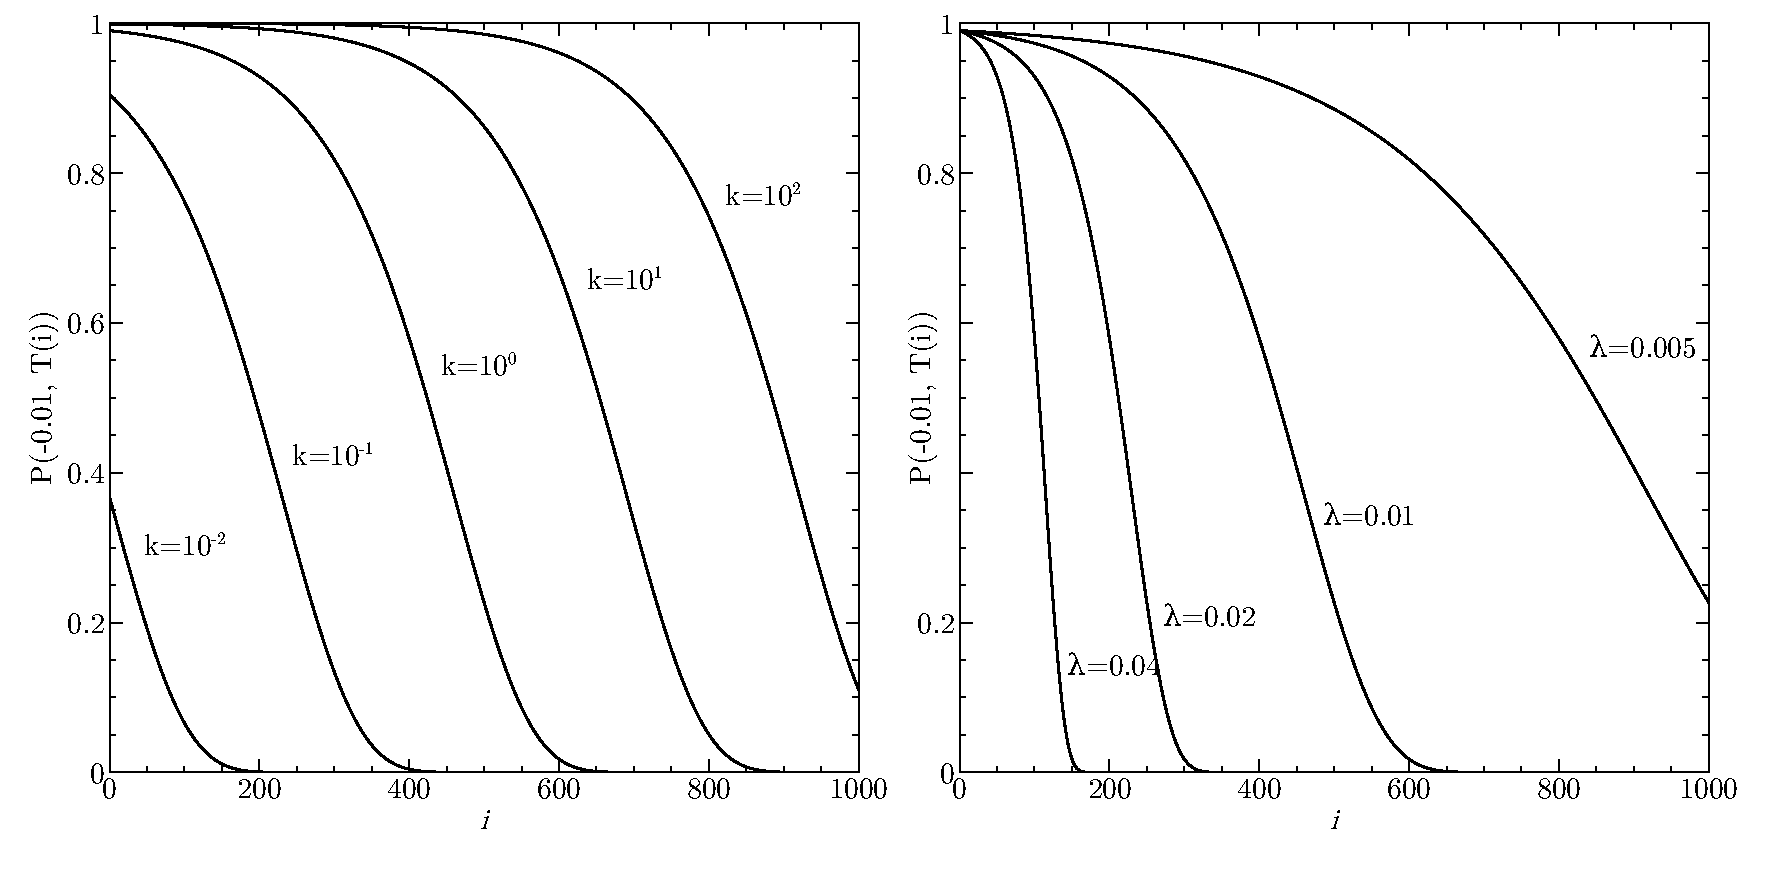
\includegraphics[width=0.99\linewidth]{../figures/SA_parameters}
\caption[Probability to accept a worse solution]{Effect of the $k$ and $\lambda$ parameters in the temperature schedule. The figures show the probability to adopt a worse solution with an energy increment $\Delta E = -0.01$ as a function of the iteration $i$. In the left figure, $\lambda$ is fixed to $\lambda=0.01$. In the right figure $k$ is fixed to $k=1$.}
\label{fig:parameters}
\end{figure}

\section{The solution space of SAGA}
We have developed and tested our method to set $k$ and $\lambda$ automatically with SAGA (Simulated Annealing Graph Aligner)~\cite{SAGA} in mind. Nevertheless, the concepts are valid for applications of simulated annealing in other domains. 

SAGA uses simulated annealing for the problem of Network Alignment. Formally, the problem of Network Alignment asks the following (at least the variant that we consider): given two graphs (also called networks) find an alignment maximizing some objective function. An alignment is a one-to-one mapping from the nodes of the smaller network to nodes of the larger network.

Thus, in SAGA solutions are alignments between two graphs. Let $G_1=(V_1,E_1)$ and $G_2=(V_2,E_2)$ be the networks. Let $n_1=|V_1|$ and $n_2=|V_2|$, with $n_1\leq n_2$. An alignment maps each node of $G_1$ to a unique node in $G_2$. The size of the search space (number of possible alignments) is
$$\prod_{i=n_2-n_1+1}^{n_2}i=\frac{n_2!}{(n_2-n_1)!}$$
This is because, given some arbitrary ordering of the nodes of $G_1$, the first one can be assigned to $n_2$ nodes, the second one to $n_2-1$ nodes, \ldots, and the last one to $n_2-n_1+1$ nodes.

Two alignments are neighbors if the only difference between them is that a mapping has changed (change neighbors) or that two mappings have swapped (swap neighbors) (see Figure~\ref{fig:operators}). Each alignment has $n_1 (n_2-n_1)$ change neighbors, and ${n_1\choose 2}$ swap neighbors. Hence, the branch factor (the number of neighbors of each alignment) is the sum of the two: $n_1 n_2 - {n_1}^2/2-n_1/2$. In particular, when the two networks have the same size there are only swap neighbors, so the branch factor is $n_1(n_1-1)/2$.

\begin{figure}
\centering
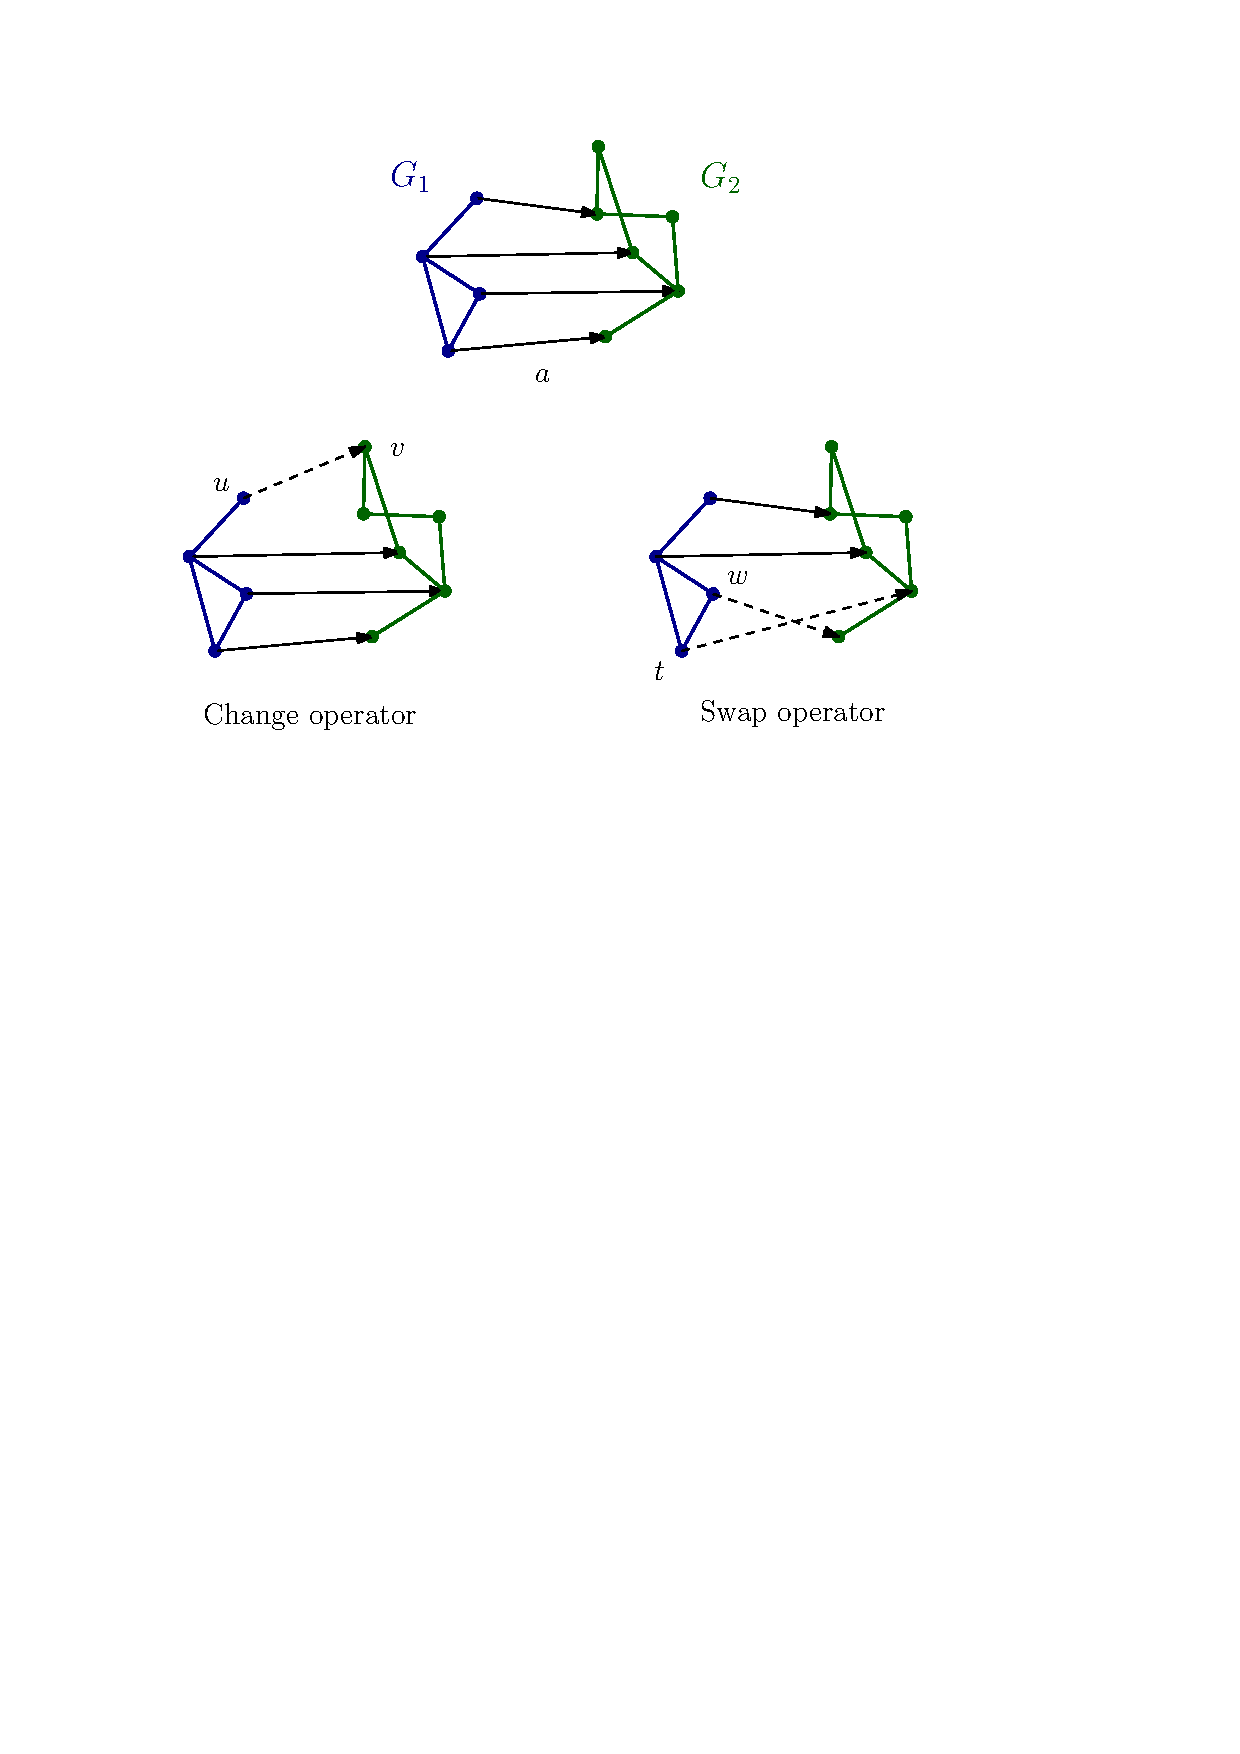
\includegraphics[width=0.7\linewidth]{../figures/operators3}
\caption{{\bf Top}: an alignment between $G_1$ on the left and $G_2$ on the right, with the alignment depicted by horizontal arrows.
{\bf Bottom left}: a {\it change} neighbor: the alignment of node $u_4$ has moved from $v_4$ to $v_5$.
{\bf Bottom right}: a {\it swap} neighbor: the alignments $(u_1,v_1)$ and $(u_2,v_2)$ have swapped to be $(u_1,v_2)$ and $(u_2,v_1)$.}
\label{fig:operators}
\end{figure}

The solution space is connected: any two alignments are connected through a path of neighbor alignments. Its diameter (maximum number of steps between two solutions) is $O(n_1)$.

Regarding the objective function, in network alignment there are several metrics of alignment quality, called \textit{measures}. Formally, a measure is a function $f(x)$ that maps alignments to the range $[0,1]$, although it can be generalized to arbitrary values in $\mathbb{R}$. A score of $1$ denotes a flawless alignment, while a score of $0$ denotes that the alignment could not be worse. However, given a measure $f$ we cannot assume that the scores of the alignments will be distributed uniformly along the range $[0,1]$. Some measures such as sequence similarity tend to have very small scores, e.g., in the range $[0,0.05]$, while for other measures even random alignments obtain scores significantly higher than zero. For instance, in one of our datasets the GO term count measure scores usually fall in the range $[0.4,0.6]$. In general, we cannot make any assumption about the mean or variance of the scores of the alignments in the solution space. For instance, an alignment with a score of 0.8 is not necessarily good, and a score that is only 0.05 better than a random alignment is not necessarily bad.

\section{Methodology}

Formally, our goal is to find the values for $k$ and $\lambda$ to maximize $f(x)$ constrained to a maximum execution time of $s$ seconds. Our input are the networks $G_1$ and $G_2$ and the measure $f$, also called objective function.

A straightforward approach would be to try a set of combinations of values of $k$ and $\lambda$, and take the pair that works best. However, there are several difficulties:
\begin{itemize}
\item The best value for $k$ and for $\lambda$ cannot be searched independently, as each one affects the other.
\item There are no clear lower or upper bound for neither $k$ nor $\lambda$. It is not clear if the search should be linear or logarithmic.
\item In order to know how well a combination of values of $k$ and $\lambda$ does, it is necessary to run SAGA and wait until the end (i.e., $s$ seconds). A temperature schedule with which SAGA finds a good alignment early on will not necessarily be the best in the end. In fact, if it starts converging too quickly, it likely means that there is not enough randomness and the final score will not be particularly good.
\item Our experiments suggest that there are no clear trends in the landscape of the solution space to guide the search easily (see Figure~\ref{fig:temperature}).
\end{itemize}

\begin{figure}
\centering
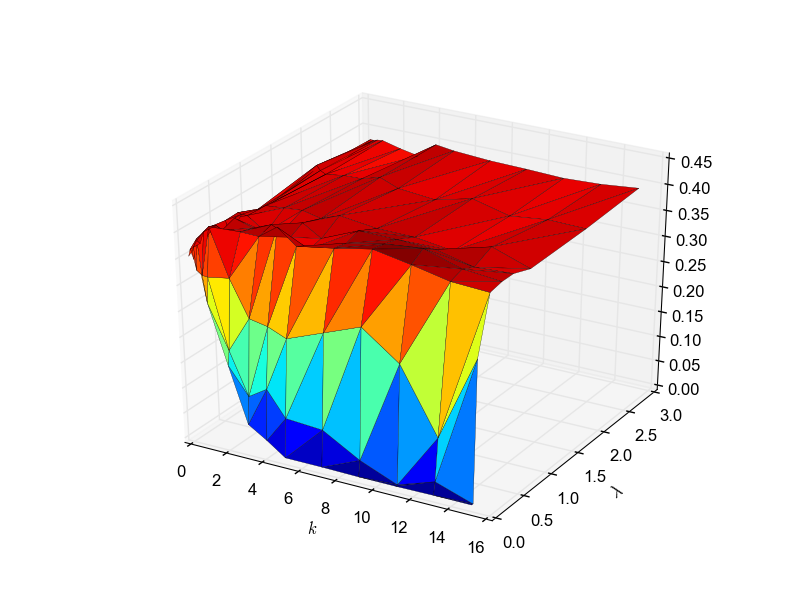
\includegraphics[width=0.99\linewidth]{../figures/temperature}
\caption[Temperature schedule]{126 one-hour runs of SAGA with yeast and human PPI networks, optimizing EC (Edge Coverage), with different values of $k$ and $\lambda$. The $z$-axis is the EC score. The values of $k$ displayed are the original values used multiplied by $2.5\cdot 10^{4}$. The values of $\lambda$ displayed are the original values used multiplied by $10^{8}$. The sudden drop for scores with $\lambda=0.1$ is because the temperature decreased so slowly that SAGA did not have time to converge in one hour.}
\label{fig:temperature}
\end{figure}

All these reasons motivated us to follow a more analytical approach. Function of the form $T(i)=k/e^{\lambda i}$, where $k$ and $\lambda$ are constants, are characterized by two points. Therefore, we only need to ``choose'' two points, and then we can set $k$ and $\lambda$ to the values that fit $T(i)$ to go through these points. The first one will be the starting point, $(0,k)$. The second point will be $(i_s,\epsilon)$, where $i_s$ is the estimated number of iterations that SAGA will make in $s$ seconds, and $\epsilon$ is the \textit{terminal temperature}, a value so small that it has allowed SAGA to converge to a local maximum. The function of the form $T(i)=k/e^{\lambda i}$ that goes through $(0,k)$ and $(i_s,\epsilon)$ has $\lambda=\log(k/\epsilon)/i_s$.

\subsection{Setting the initial temperature}

First, we focus on how to find $k$, the initial temperature. Let $S_R$ denote the random variable ``score of a random alignment'' (a random alignment is a just an alignment taken randomly and uniformly from the solution space). Moreover, let $S_t$ be the random variable ``score obtained when running SAGA for $n_1\cdot n_2$ iterations\footnote{The number $n_1\cdot n_2$ of iterations is a rather arbitrary value. In practice, it suffices that it is ``large enough''.} and the temperature fixed to $t$''. We work under the assumption that these random variables follow a normal distribution. We tested these hypothesis with the Shapiro-Wilk normality test, and we were not able to reject it, which means that the data seems to follow a normal distribution. This assumption might not hold when optimizing certain measures, but it is true for most typical ones. If $t$ is high enough, then $S_t\sim S_R$. In other words, with high temperatures the search is random and does not do any ``useful work''. Let $t_k$ denote the smallest $t$ such that $S_t\sim S_R$.

Let $t^*$ denote the ideal starting temperature. Clearly, $t^*\leq t_k$. This is because if $t^*>t_k$, SAGA will just wander randomly through the solution space until $T(i)=t_k$, hence wasting execution time. On the other hand, it may be the case that $t^*<t_k$, but within the range $(0,t_k]$, we think that $t_k$ is the best candidate to initial temperature, for the following reasons:
\begin{itemize}
\item Given that $t^*\leq t_k$, by setting the initial temperature to $t_k$, it will eventually reach $t^*$.
\item The temperature decreases at an exponential rate, which limits the wasted execution time for overestimating the ideal initial temperature.
\item It agrees with the intuition that at the beginning, SAGA should start moving randomly.
\end{itemize}

The issue is how to find $t_k$. First, we define a function $\mbox{random?}(t)$, which, given a temperature $t$, determines if $S_t\sim S_R$. To do this, first we estimate the parameters of the normal distribution of $S_R$ (the mean $\mu$ and the standard deviation $\sigma$), with a sample of 100 scores from random alignments. Then, we run SAGA with temperature fixed to $t$ for $n_1\cdot n_2$ iterations and test the hypothesis that the obtained score $x$ belongs to $S_R$. If the p-value (i.e., the fraction of scores belonging to $S_R$ smaller than $x$) is $>0.999999$, $\mbox{random?}(t)$ returns no. If the p-value is $<0.999999$ but $>0.99$, we make $5$ additional runs of SAGA with the same fixed temperature. Only if the score of all five runs obtain p-values $>0.99$, $\mbox{random?}(t)$ returns no. In any other instance, it returns yes.

Note that the function $\mbox{random?}(t)$ can have false positives (scores that come from not random alignments are classified as random) as well as false negatives (scores that come from random alignments are classified as not random). %However, it was designed specifically to prevent false negatives, because, as we will discuss later, we consider that false negatives are less detrimental.

Next, we discuss how to use $\mbox{random?}(t)$ to find $t_k$. Our goal is to find an interval $(t_l,t_h)$, with $0<t_l<t_h$, such that $t_k\in(t_l,t_h)$, i.e., $\mbox{random?}(t_l)=\mbox{false}$ and $\mbox{random?}(t_h)=\mbox{true}$, and minimizing its length $t_h-t_l$. To obtain it, we start with the range $t_l=0,t_h=1$. It is not guaranteed that $t_k<1$. Thus, we test $\mbox{random?}(1)$, i.e., $\mbox{random?}(t_h)$. In the event that $\mbox{random?}(t_h)=\mbox{false}$, we double $t_h$. We repeat this process until $\mbox{random?}(t_h)=\mbox{true}$. Then, we can set $t_l=t_h/2$, as we would have obtained $\mbox{random?}(t_h/2)=\mbox{false}$ in the previous step.

Now that the interval satisfies the constraint that $t_k\in(t_l,t_h)$, we minimize its length doing a logarithmic binary search. At each step, we find an intermediate value $t_m$ as follows. First we transform $t_h$ and $t_l$ to a logarithmic space applying the function $f(x)=\log_2(x+1)$. We apply the logarithm to $x+1$ instead of $x$ because $\log_2(0)$ is undefined. Then, we find the mid-point in the logarithmic space: $t_m'=(f(t_h)+f(t_l))/2$. Finally, we undo the transformation: $t_m=f^{-1}(t_m')$, where $f^{-1}(x)=2^{x}-1$. We test $\mbox{random?}(t_m)$. If $\mbox{random?}(t_m)=\mbox{true}$, we set $t_l=t_m$. Otherwise, we set $t_h=t_m$.

We narrow the starting range $(t_l,t_h)$ by doing a total of 10 iterations. Once we have the final interval, we set $k=t_h$, possibly overestimating $t_k$, which we consider preferable to underestimating it.



\subsection{Setting the terminal temperature}

We have seen how to determine $(0,k)$. The second point that we have to determine is $(i_s,\epsilon)$. In order to determine $i_s$, the estimated number of iterations that SAGA will make in $s$ seconds (the execution time), we first estimate the number of iterations per second of SAGA. We run SAGA with fixed temperature $0$ until it stagnates at a local maximum (we consider that SAGA has stagnated if it goes $10^7+\log(m)$ iterations without improving, where $m={n_2!}/{(n_2-n_1)!}$ is the size of the search space, and $\log(m)$ is approximated with Stirling's approximation). Then, we divide the number of iterations that it took by the total execution time in seconds. This gives us the average number of iterations per second among the complete spectrum of alignments, from random ones to ones in local maximums. We do this because the number of iterations per second at the beginning, when there is plenty of movement through the solution space, might differ from latter stages, although according to our observations it does not vary much. Our implementation of SAGA performs in the order of $10^6$ iterations per second with networks with thousands of nodes, tens of thousands of edges, and most typical objective functions such as EC (Edge Coverage) and S3 (Symmetric Substructure Score). Once we have an estimate of the number of iterations per second $i$, we set $i_s=i\cdot s$.

At iterations $i_s$, we want the temperature to be so low that SAGA converges to a local maximum. However, $T(i)$ never reaches $0$, it approaches it asymptotically (see Figure~\ref{fig:temp}). If we run SAGA with a functional temperature schedule, it will start accepting plenty of worse solutions, and it will reduce this number as temperature decreases. We say the temperature has reached ``practically zero'' when the expected number of accepted worse neighbors per second is $1$. We consider that the temperature should reach this point at iteration $i_s$.

Note that with a functional temperature schedule, when the temperature reaches the ``practically zero'' threshold, the current alignment has almost converged. The expected number of accepted worse neighbors per second changes depends on the alignment (a good alignment will have a higher score difference with its neighbors than a random one). Thus, $\epsilon$ should be the ``practically zero'' temperature for alignments that are close to local maximum. In order to find $\epsilon$, we define a function $\mbox{expected}(t)$ which, given a temperature $t$, returns the expected number of accepted worse solutions per second with temperature fixed to $t$, and starting with an alignment that is at or close to a local maximum. Therefore, we are looking for the temperature $t_0$ such that $\mbox{expected}(t_0)=1$. We compute $\mbox{expected}(t)$ by first running SAGA with temperature fixed to 0 until it converges (recall that we consider that it has converged if it goes $10^7+\log(m)$ iterations without improving, where $m$ is the size of the search space). This gives us an alignment that is at a local maximum, thus resembling the kind of alignments that we will find at iteration $i_s$. Then, we let it run for one more second, and store all the negative score increments $s_1, \ldots, s_n$. We then use this sample of energy increments to compute $\mbox{expected}(t)$:
$$\mbox{expected}(t)=\sum_{i=1}^n P(s_i, t)=\sum_{i=1}^n e^{s_i/t}$$
Solving the equation $\mbox{expected}(t)=1$ for $t$ analytically is computationally hard. However, since $\mbox{expected}(t)$ is monotonically increasing with $t$, the point $\mbox{expected}(t)=1$ can be approximated numerically. We use the bisection method.

As opposed to the case of the search for $t_k$ in the previous section, this time we have an analytical lower and upper bound for $t_0$. Let $s_{min}=\min(s_i)$ and $s_{max}=\max(s_i)$. As all the $s_i$ are smaller than zero, we have $e^{s_{min}/t_0}\le e^{s_i/t_0}\le e^{s_{max}/t_0}$ for all $s_i$. Hence,
$$e^{s_{min}/t_0} \le \dfrac{\sum_{i=1}^n e^{s_i/t_0}}{n}\le e^{s_{max}/t_0}$$
and given that $\sum_{i=1}^n e^{s_i/t_0}=\mbox{expected}(t_0)=1$, we have that $e^{s_{min}/t_0}\le 1/n\le e^{s_{max}/t_0}$, or equivalently
$$\frac{|s_{max}|}{\ln(n)} \le t_0 \le \frac{|s_{min}|}{\ln(n)}$$

We do a total of 100 binary search iterations in the obtained range to approximate $\epsilon$.

\section{Results}

Tables~\ref{tab:s3},~\ref{tab:s32}, and~\ref{tab:nc} compare the results obtained by SAGA with and without automatic temperature schedule. For the results without, we use those reported in~\cite{SAGA}, where $k$ and $\lambda$ were chosen by hand. In both cases, the objective function of SAGA was S3 (Symmetric Substructure Score). For a description of the datasets and objective functions, as well as a comparison between SAGA and other methods, see~\cite{SAGA}.

In the tables, ``SAGA'' corresponds to the results reported in~\cite{SAGA}. The total execution time with restarts was 4h. ``SAGA*'' corresponds to the results with automatic temperature schedule, no restarts, and a total execution time of 1h (without counting the time spent finding $k$ and $\lambda$, which usually is a few minutes).

The results with automatic restart schedule are better in almost every case, and with a smaller execution time. Moreover, it removes the burden of doing trial and error to find $k$ and $\lambda$ from the user, improving SAGA's usability.
  
\begin{table}
\centering
\caption{S3 comparison on the BioGRID dataset and Yeast-Human dataset.}
\label{tab:s3}
\begin{tabular}{llll}
G1          & G2            & SAGA  & SAGA* \\ \hline
yeast       & human         & 0.396240 & 0.384941     \\
RNorvegicus & SPombe        & 0.498136 & 0.504969     \\
RNorvegicus & CElegans      & 0.478528 & 0.482744     \\
RNorvegicus & MMusculus     & 0.597479 & 0.617450     \\
RNorvegicus & AThaliana     & 0.642179 & 0.671829     \\
RNorvegicus & DMelanogaster & 0.522690 & 0.536999     \\
SPombe      & CElegans      & 0.407804 & 0.409136     \\
SPombe      & MMusculus     & 0.487651 & 0.510904     \\
SPombe      & AThaliana     & 0.556653 & 0.565305     \\
SPombe      & DMelanogaster & 0.487717 & 0.499241     \\
CElegans    & MMusculus     & 0.410471 & 0.437717     \\
CElegans    & AThaliana     & 0.436861 & 0.457653     \\
MMusculus   & DMelanogaster & 0.351600 & 0.370885     \\
AVG         &               & 0.482616 & 0.496136    
\end{tabular}
\end{table}

\begin{table}
\centering
\caption{S3 comparison on the Noisy yeast dataset.}
\label{tab:s32}
\begin{tabular}{llll}
G1   & G2    & SAGA  & SAGA* \\ \hline
0syn & 5syn  & 0.923346 & 0.941069     \\
0syn & 10syn & 0.871507 & 0.889309     \\
0syn & 15syn & 0.850083 & 0.847027     \\
0syn & 20syn & 0.820260 & 0.803941     \\
0syn & 25syn & 0.774304 & 0.789906     \\
AVG  &       & 0.847900 & 0.854250    
\end{tabular}
\end{table}

 \begin{table}
 \centering
 \caption{NC (Node Correctness) comparison on the Noisy yeast dataset.}
 \label{tab:nc}
 \begin{tabular}{llll}
 G1   & G2    & SAGA  & SAGA* \\
 0syn & 5syn  & 0.742032 & 0.775896 \\
 0syn & 10syn & 0.676295 & 0.740040 \\
 0syn & 15syn & 0.711155 & 0.710159 \\
 0syn & 20syn & 0.692231 & 0.667331 \\
 0syn & 25syn & 0.641434 & 0.719124 \\
 AVG  &       & 0.692629 & 0.722510
 \end{tabular}
 \end{table}


\section{Future work}

Despite the capacity of simulated annealing to escape local maximums, the final result is often affected in great measure by the first steps of the algorithm. Some mappings may become ``locked'' because undoing them would cause a large score decrease, although there exist better choices for these nodes. Thus, it often benefits from implementing some kind of restart scheme, so that unpromising alignments are discarded early on. This presents the challenge of how to detect promising runs early, and how to distribute execution time among runs.

\bibliographystyle{abbrv}
\bibliography{../Bibliography}



\end{document}
